\chapter{Banco de Questões}
\label{cap6}

\atencao{Atenção: Este material ainda não foi totalmente adaptado para o Moodle 2.4, contendo 
algumas (poucas) Figuras do Moodle 2.3. Esperamos finalizar em breve este documento para o Moodle 2.4. \bigskip}


Localizado no bloco Configurações do curso, o banco de questões é divido em quatro abas conforme mostrado abaixo. O banco de questões é usado para criar uma coleção de perguntas permitindo o compartilhamento de perguntas que podem ser utilizadas em outros questionários da disciplina ou de outros cursos. As questões são organizadas em Categorias, podendo ser transferidas para a atividade questionário de forma manual ou aleatória. 

\section{Categorias}
Para organizar e facilitar a identificação do tipo de questão(ões) da disciplina, pode-se criar ou editar uma ou mais categorias. Estas são separadas numa hierarquia, em contextos diferentes, como mostra a Figura \ref{fig:cap6_26}

\begin{figure}[htbp]
 \begin{center}
 \fbox{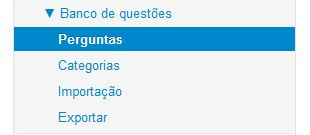
\includegraphics[width=0.5\textwidth]{imagem/cap6/fig26.jpg}}
  \caption{Menu Categoria}
  \label{fig:cap6_26}
 \end{center}
\end{figure}

\textbf{Padrão para Nome do Curso:} as questões são disponíveis para todos os módulos de atividades em uma disciplina.

\textbf{Padrão para Miscelânea:} as questões são disponíveis para todos os módulos de atividades em uma disciplina, como também em uma categoria de cursos. Neste exemplo, a disciplina está inserida na categoria de cursos Miscelânea.

\textbf{Padrão para Sistema: }as questões são disponíveis para todos os módulos de atividades e cursos do Moodle.

Cada contexto tem sua própria hierarquia, geralmente aparecerá em negrito cada categoria. É chamado de categoria pai, aquela onde um item deve ser incluído. Deste modo, para adicionar uma categoria, basta escolher a categoria pai, de acordo com as categorias que o professor tem permissão de acesso, que será inserida e atribuir um nome, conforme mostrado na Figura \ref{fig:cap6_27}.

\begin{figure}[htbp]
 \begin{center}
 \fbox{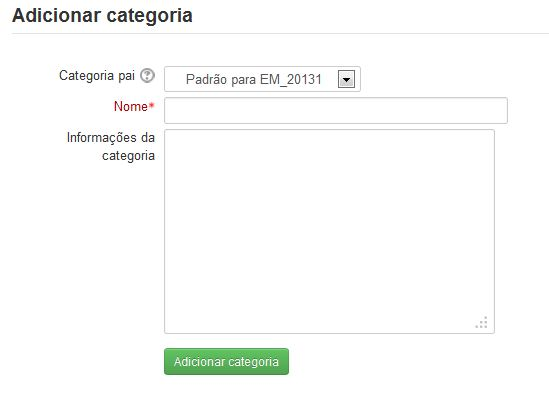
\includegraphics[width=0.4\textwidth]{imagem/cap6/fig27.jpg}}
  \caption{Adicionando Categoria}
  \label{fig:cap6_27}
 \end{center}
\end{figure}

Para finalizar, clicar em  \textbf{Add Category}.
Ao criar uma categoria, ela aparecerá no contexto da categoria pai selecionada. No exemplo abaixo, foi criada a categoria Questionário dentro do contexto Padrão para Curso (Figura \ref{fig:cap6_28}). 

\begin{figure}[htbp]
 \begin{center}
 \fbox{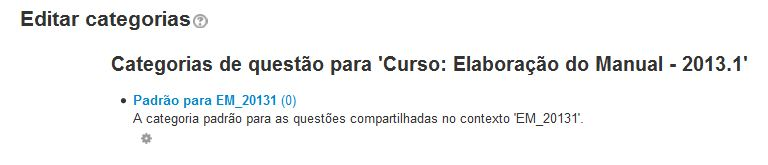
\includegraphics[width=0.4\textwidth]{imagem/cap6/fig28.jpg}}
  \caption{Editar Categoria}
  \label{fig:cap6_28}
 \end{center}
\end{figure}

\section{Quadro de Notas}

\subsection{Categoria e Itens}

No quadro de notas do Moodle, conforme mencionado anteriormente, o professor manipula \textbf{itens de nota} e \textbf{categorias de nota}. Sua visibilidade, ordem e agregação podem ser definidas sem alterar as respectivas propriedades das atividades na página principal da disciplina. Por exemplo, o professor pode ocultar as atividades na disciplina à medida que seu prazo esgotar, o oposto também pode ser feito deixando as notas visíveis conforme o prazo de publicação da mesma estiver em aberto.

Essa manipulação é feita na página \textbf{Categorias e itens} do quadro de notas. Ela possui duas versões de visualização \textbf{Visão simples} e \textbf{Visão completa}. A diferença entre estes modos de visualização é o número de opções de configuração apresentados na tela principal para o professor (ver Figuras \ref{fig:cap6_1} e \ref{fig:cap6_6}). Todas as opções exibidas estão também disponíveis, para o item ou categoria de nota em sua página de configuração, acessada ao clicar no ícone de edição 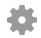
\includegraphics[width=0.02\textwidth]{imagem/cap5/fig7.jpg} (\textbf{engrenagem}), da coluna \textbf{ações}.

Na página de visualização simples, por exemplo, pode-se:

\begin{itemize}
 \item Definir o resultado da agregação para as categorias;
 \item Definir se uma atividade contará apenas como crédito extra;
 \item Visualizar a nota máxima de cada atividade;
 \item Mover (ordenar) os itens e categorias;
 \item Ocultar ou deixar visível aos alunos;
 \item Travar ou destravar uma atividade.
\end{itemize}

\begin{figure}[htbp]
 \begin{center}
 \fbox{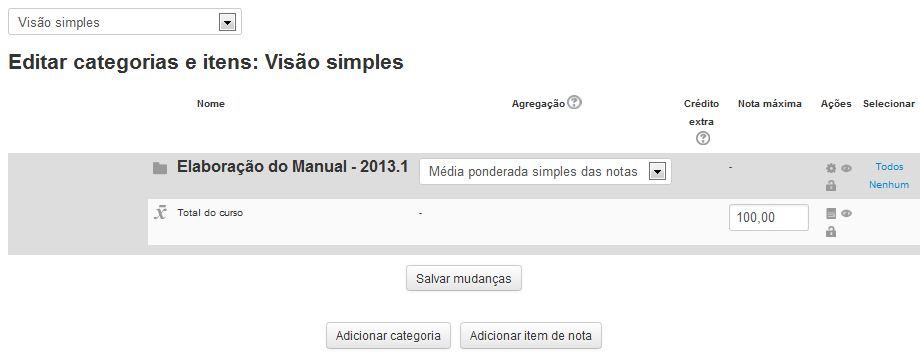
\includegraphics[width=0.5\textwidth]{imagem/cap6/fig1.jpg}}
  \caption{Categoria e Itens (Visão simples)}
  \label{fig:cap6_1}
 \end{center}
\end{figure}

\begin{figure}[htbp]
 \begin{center}
 \fbox{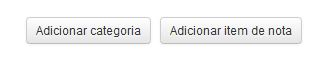
\includegraphics[width=0.5\textwidth]{imagem/cap6/fig2.jpg}}
  \caption{Categoria e Itens (Visão simples)}
  \label{fig:cap6_2}
 \end{center}
\end{figure}

\subsection{Categoria de nota}
Ao final da página, podemos adicionar uma categoria de notas, itens de notas e item de resultado da aprendizagem. Uma \textbf{categoria de nota} é um elemento que contém um conjunto de atividades. Para cria-la, clicamos no botão \textbf{Adicionar categoria} Figura \ref{fig:cap6_3}, que redirecionará para página de configuração da categoria, Figura \ref{fig:cap6_4}.

\begin{figure}[htbp]
 \begin{center}
 \fbox{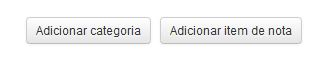
\includegraphics[width=0.5\textwidth]{imagem/cap6/fig3.jpg}}
  \caption{Botões de Adicionar categoria, Item de Nota e Resultado da aprendizagem}
  \label{fig:cap6_3}
 \end{center}
\end{figure}

\begin{figure}[htbp]
 \begin{center}
 \fbox{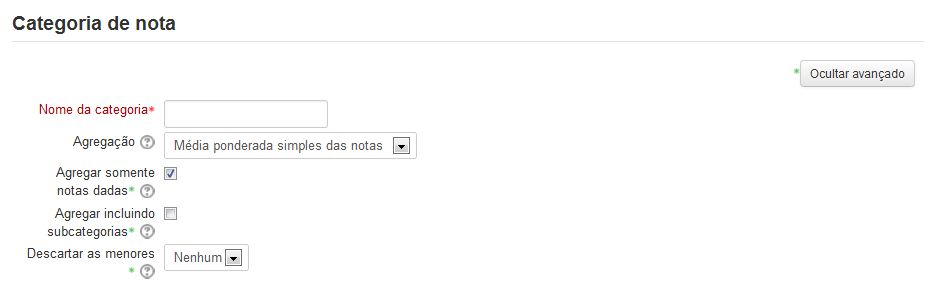
\includegraphics[width=0.5\textwidth]{imagem/cap6/fig4.jpg}}
  \caption{Adicionar categoria}
  \label{fig:cap6_4}
 \end{center}
\end{figure}

A princípio devemos informar o \textbf{nome da categoria} que será visualizada pelos alunos na planilha de notas.

A \textbf{agregação} de uma categoria é o resultado que ela retorna (exibe) para aquele determinado conjunto de atividades (ex. uma soma, uma média).

Os tipos de agregação são descritos a seguir, considerando sempre o valor máximo da categoria como 100 e o mínimo como zero. Multiplicar o resultado percentual pelo valor máximo (neste caso 100) é suficiente para se obter o resultado final da agregação:

\subsubsection{Média das notas}
O resultado é a soma de todas as notas dividida pelo número de notas.

\begin{figure}[htbp]
 \begin{center}
 \fbox{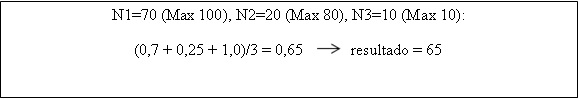
\includegraphics[width=0.6\textwidth]{imagem/cap6/fig5.jpg}}
  \label{fig:cap6_5}
 \end{center}
\end{figure}

\subsubsection{Média ponderada das notas}
Pode ser atribuído um peso para cada nota, que é multiplicado pela respectiva nota no cálculo da média. A soma das notas ponderadas é divida pela soma dos pesos.

\begin{figure}[htbp]
 \begin{center}
 \fbox{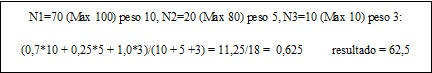
\includegraphics[width=0.6\textwidth]{imagem/cap6/fig6.jpg}}
  \label{fig:cap6_6}
 \end{center}
\end{figure}

\subsubsection{Média ponderada simples das notas}
A diferença para a Média Ponderada é que o peso é calculado como Nota máxima - Nota mínima para cada item. Uma tarefa de 100 pontos tem peso 100, enquanto que uma de 10 pontos tem peso 10 (considerando a nota mínima como zero).

\begin{figure}[htbp]
 \begin{center}
 \fbox{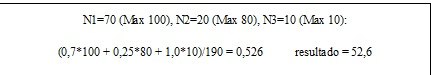
\includegraphics[width=0.6\textwidth]{imagem/cap6/fig7.jpg}}
  \label{fig:cap6_7}
 \end{center}
\end{figure}

\subsubsection{Média das notas (com pontos extras)}
Média aritmética com pontuação extra. Uma estratégia de agregação antiga e ultrapassada, mantida atualmente apenas por questões de compatibilidade com algumas atividades antigas.
\subsubsection{Mediana das notas}
A nota do meio (ou a média de duas notas do meio, caso o número seja par), obtida após ordenação das notas. A vantagem sobre a média é que ela não é afetada por valores atípicos (notas que estão muito longe da média).

\begin{figure}[htbp]
 \begin{center}
 \fbox{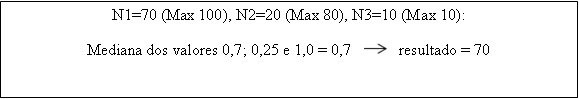
\includegraphics[width=0.6\textwidth]{imagem/cap6/fig8.jpg}}
  \label{fig:cap6_8}
 \end{center}
\end{figure}

\subsubsection{Menor nota}
O resultado é a menor nota após a normalização.

\begin{figure}[htbp]
 \begin{center}
 \fbox{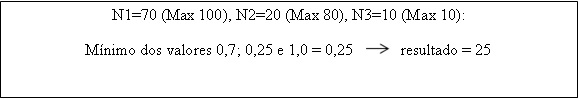
\includegraphics[width=0.6\textwidth]{imagem/cap6/fig9.jpg}}
  \label{fig:cap6_9}
 \end{center}
\end{figure}

\subsubsection{Maior nota}
O resultado é a maior nota após a normalização.

\begin{figure}[htbp]
 \begin{center}
 \fbox{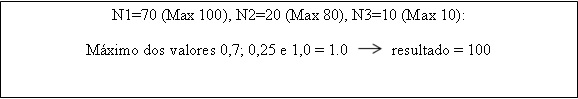
\includegraphics[width=0.6\textwidth]{imagem/cap6/fig10.jpg}}
  \label{fig:cap6_10}
 \end{center}
\end{figure}

\subsubsection{Moda das notas}
A moda é a nota que ocorre com mais frequência. A vantagem sobre a média é que ela não é afetada por valores atípicos (notas que estão muito longe da média). Entretanto, ele perde significado quando há mais de uma nota mais frequente (apenas uma será escolhida), ou quando todas as notas são distintas entre si.

\begin{figure}[htbp]
 \begin{center}
 \fbox{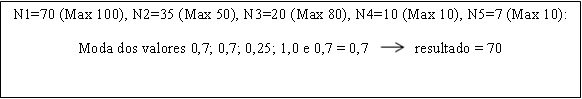
\includegraphics[width=0.6\textwidth]{imagem/cap6/fig11.jpg}}
  \label{fig:cap6_11}
 \end{center}
\end{figure}

\subsubsection{Soma das notas}
A soma de todas as notas. As escalas são ignoradas. Esse é o único tipo de agregação que não converte internamente as notas para percentagem (normalização). A Nota Máxima do item associado à categoria é calculada automaticamente como a soma dos máximos de todos os itens agregados.

\begin{figure}[htbp]
 \begin{center}
 \fbox{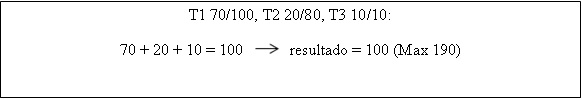
\includegraphics[width=0.6\textwidth]{imagem/cap6/fig12.jpg}}
  \label{fig:cap6_12}
 \end{center}
\end{figure}

Ao clicar no botão \textbf{Mostrar avançado}, ainda na tela de Adicionar nova categoria, nos deparamos com a opção Incluir resultado da aprendizagem na agregação, o que significa que ao selecionarmos essa opção podemos conduzir a nota final diferente da desejada, de forma que você tem a opção de incluí-los ou deixá-los de fora.

No item Agregar incluindo subcategorias a agregação será feita normalmente só com a categoria descendente imediata, mas também é possível agregar avaliações em todas as subcategorias, excluindo outras avaliações agregadas. Já em Descartar as menores, permite desconsiderar as notas mais baixas, classificando essas notas como o valor escolhido para essa opção.

Seguindo a mesma página, é preciso preencher os campos relacionados ao Total da categoria, conforma na Figura abaixo.

\begin{figure}[htbp]
 \begin{center}
 \fbox{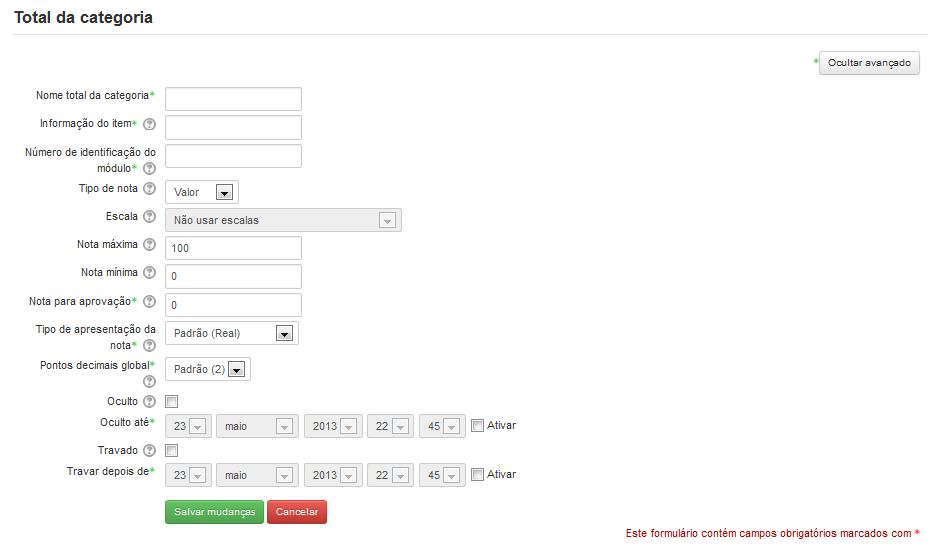
\includegraphics[width=0.6\textwidth]{imagem/cap6/fig13.jpg}}
  \caption{Adicionar categoria}
  \label{fig:cap6_13}
 \end{center}
\end{figure}
Todos os itens que acompanham o sinal de asterisco (*) são itens dispensáveis, ou seja, o seu preenchimento não é obrigatório.

\begin{itemize}
 \item \textbf{Nome total da categoria(\*):} define um rótulo para o total da categoria criada.
 \item \textbf{Informação do Item(\*):} espaço destinado para adicionar informações sobre o item. Esse texto não aparece em nenhum outro espaço.
 \item \textbf{Número identificação do módulo(\*):} definir uma identificação, que pode também ser uma abreviatura, é uma maneira de identificar a atividade para propósitos de cálculo na planilha de notas. Se a atividade não é utilizada em nenhum cálculo de notas, o campo pode ficar em branco. O número de identificação do módulo para um item de nota baseado em atividades é configurado na página de configurações das atividades.
 \item \textbf{Tipo de nota:} neste campo você define o tipo de nota que será utilizado na categoria, dentre as seguintes opções: Nenhum (sem notas), Valor (de forma numérica permite configurações de máximo e mínimo), Escala (permite configurações de escala) ou Texto (somente feedback).
 \item \textbf{Escala:} caso tenha escolhido a opção Escala no campo Tipo de Nota, selecione um tipo de escala.
 \item Nota máxima: caso tenha escolhido a opção Valor na opção Tipo de Nota, neste campo é possível determinar um valor máximo para este Item de Avaliação.
 \item \textbf{Nota mínima:} caso tenha escolhido a opção Valor na opção Tipo de Nota, neste campo é possível determinar um valor mínimo para este Item de Avaliação.
 \item \textbf{Nota para aprovação(\*):} neste campo é possível determinar um valor que os alunos precisam igualar ou exceder para serem aprovados neste item de avaliação (atingir a suficiência).
 \item \textbf{Tipo de apresentação da nota(\*):} define como as notas serão mostradas no relatório de notas e nos relatórios do aluno, escolhendo dentre as seguintes opções: Real (nota), Porcentagem ou Letra (conceito).
 \item Pontos decimais global(\*): especifica o número de casas decimais em que a nota será mostrada. Essa configuração não possui efeito nos cálculos de notas, que são feitos com uma exatidão de 5 casas decimais.
 \item Oculto: neste campo você define se as notas serão ou não ocultadas para os alunos, geralmente após o término da atividade e no processo de avaliação.
 \item \textbf{Oculto até (\*):} estabelece um prazo até que as notas sejam liberadas aos alunos.
 \item \textbf{Travado:} determina se a avaliação não aceita atualização automática a partir da atividade a que ela está ligada. Normalmente esta opção é habilitada (Travado) assim que a atividade termina e as submissões não são mais aceitas.
 \item \textbf{Travar depois de (\*):} define a data posterior da qual as notas serão destravadas. Geralmente essa data é configurada para o término da atividade e o começo do processo de avaliação.
\end{itemize}
\textbf{Categoria Pai:} Posiciona a categoria de notas na raiz ou em categorias pré-existentes.
Realizados esses procedimentos, clique no botão Salvar mudanças ou Cancelar.
Ao retornar para página principal de Categorias e Itens (Figura \ref{fig:cap6_14}), percebemos que na categoria criada, podemos definir o tipo de agregação, selecionando o menu com a seta ao lado.
\begin{figure}[htbp]
 \begin{center}
 \fbox{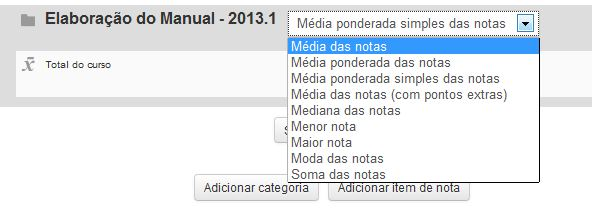
\includegraphics[width=0.6\textwidth]{imagem/cap6/fig14.jpg}}
  \caption{Definir tipo de agregação}
  \label{fig:cap6_14}
 \end{center}
\end{figure}

Uma ou mais atividades podem ser marcadas como \textbf{crédito extra} para o resultado da categoria na qual estiverem inseridas se a agregação escolhida for \textbf{soma das notas} ou \textbf{média ponderada simples}. Isto é feito clicando-se na caixa da respectiva atividade na coluna \textbf{Crédito extra}.

Uma atividade assim marcada não terá seu valor acrescido ao valor máximo da categoria. Suponha uma categoria cuja agregação seja \textbf{soma das notas} e que contenha 4 atividades de valor 10. Se uma delas for marcada como crédito extra o resultado máximo da categoria seria 30, mesmo para os alunos que ultrapassassem este valor na soma individual das atividades. O crédito extra, desta forma, eleva a média das notas dos alunos para uma categoria.

Na coluna \textbf{ações} estão disponíveis as opções de \textbf{editar}, \textbf{excluir}, \textbf{mover}, \textbf{ocultar/mostrar} e \textbf{travar/destravar}.
\begin{figure}[htbp]
 \begin{center}
 \fbox{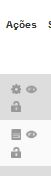
\includegraphics[width=0.07\textwidth]{imagem/cap6/fig15.jpg}}
  \caption{Coluna Ações}
  \label{fig:cap6_15}
 \end{center}
\end{figure}

Ao clicar em \textbf{editar} 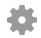
\includegraphics[width=0.03\textwidth]{imagem/cap5/fig7.jpg} (\textbf{engrenagem}), em um item ou categoria de nota, uma nova janela se abrirá com as opções de configuração para aquele elemento. Por exemplo, clicando no botão editar do item \textbf{Apresentação} (Figura \ref{fig:cap6_15}) e a seguir no botão mostrar avançado no canto superior direito da tela, mostrará as configurações avançadas do item ou categoria de nota.

O ícone de interrogação circundada 
\includegraphics[width=0.03\textwidth]{imagem/cap6/fig17.jpg} é um link que abre uma janela explicativa para cada propriedade disponível para o item escolhido.

A opção de \textbf{excluir}  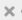
\includegraphics[width=0.03\textwidth]{imagem/cap6/fig18.jpg} está disponível apenas para alguns itens de nota ou os itens criados diretamente na página de categorias e itens (como será visto mais adiante).

A opção \textbf{mover} 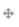
\includegraphics[width=0.03\textwidth]{imagem/cap6/fig19.jpg}  permite que um item de nota possa ter sua posição alterada. Ao clicar no link para o item de nota \textbf{Apresentação} na Figura \ref{fig:cap6_16}, por exemplo, teremos a seguinte tela.

\begin{figure}[htbp]
 \begin{center}
 \fbox{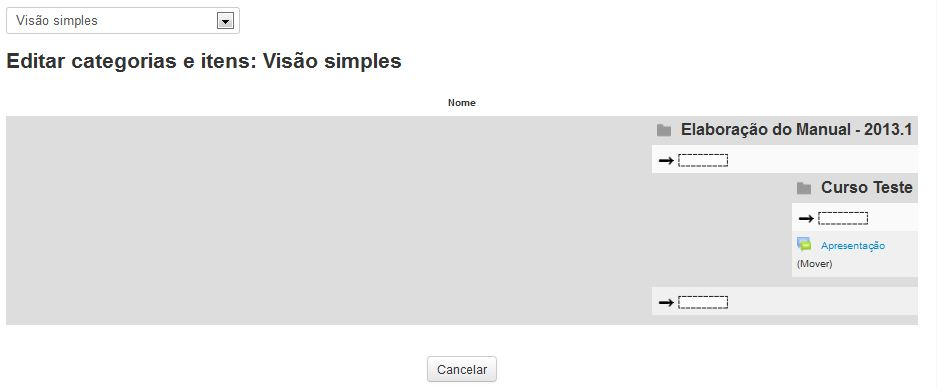
\includegraphics[width=0.6\textwidth]{imagem/cap6/fig16.jpg}}
  \caption{Coluna Ações}
  \label{fig:cap6_16}
 \end{center}
\end{figure}
O item fica destacado e com a palavra “mover” à sua frente. Basta clicar num dos espaços quadriculados para mover o item para àquele espaço. O professor pode, por exemplo, alocar todas as tarefas juntas, a seguir todos os fóruns e assim por diante. Caso o professor desista de mover o item, basta clicar no botão \textbf{Cancelar}.

\subsection{Item de notas}
Para acrescentar um item de avaliação ou notas, o qual representa criar uma nova coluna de nota na planilha, sem estar vinculado a uma atividade ou sala de entrega de tarefas, clique no botão Adicionar item de nota que o remeterá para a página de configuração da mesma. (Figura \ref{fig:cap6_20})

\begin{figure}[htbp]
 \begin{center}
 \fbox{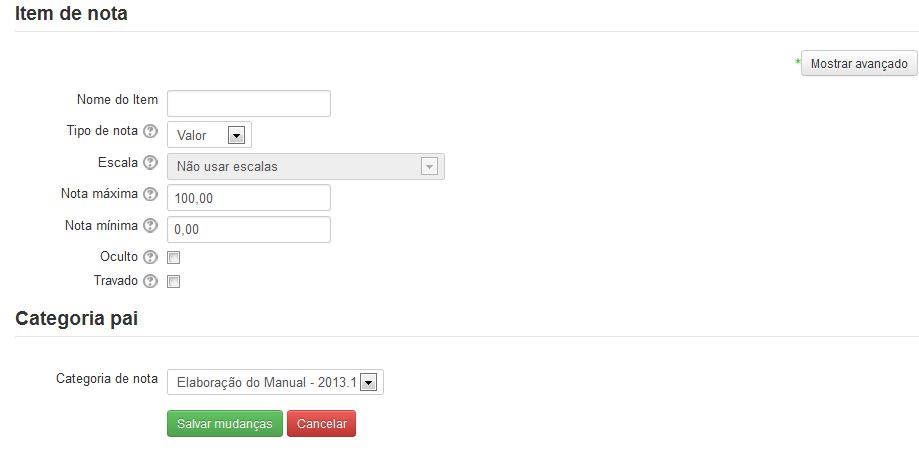
\includegraphics[width=0.6\textwidth]{imagem/cap6/fig20.jpg}}
  \caption{Configuração do Item de notas}
  \label{fig:cap6_20}
 \end{center}
\end{figure}
Alguns campos são bem semelhantes aos citados nas configurações de Categorias de notas, portanto, definimos de maneira sucinta as principais propriedades e opções do Item de notas.

\begin{itemize}
 \item \textbf{Nome do Item:} define um nome ou título do item de nota.
 \item \textbf{Tipo de nota:} define o tipo de nota que será utilizado, dentre as seguintes opções: Nenhum (sem notas), Valor (de forma numérica permite configurações de máximo e mínimo), Escala (permite configurações de escala) ou Texto (somente feedback).
 \item \textbf{Escala:} Item dependente do Tipo de nota, caso tenha selecionado a opção Escala, o campo será habilitado permitindo que os itens estejam visíveis na página de atualização de atividades.
 \item \textbf{Nota máxima:} caso tenha escolhido a opção Valor no campo Tipo de Nota, será possível determinar um valor máximo para este Item de Avaliação.
 \item \textbf{Nota mínima:} caso tenha escolhido a opção Valor no campo Tipo de Nota, será possível determinar um valor mínimo para este Item de Avaliação.
 \item \textbf{Oculto:} permite ocultar a nota para os alunos. Geralmente é utilizado no período de avaliação.
 \item \textbf{Travado:} não permite atualização automática da nota até que seja destravada. Geralmente essa opção é utilizada quando cessa o período de conclusão das atividades e as submissões não são mais aceitas.
 \end{itemize}

\subsection{Resultado de aprendizagem}

Retornando a página principal de Categorias e Itens, próximo passo é acrescentar um item de resultado da aprendizagem, primeiramente é necessário já ter adicionado um Resultado de aprendizagem, localizado no menu configurações (veja a Figura \ref{fig:cap6_21}). Este item será um parecer geral sobre o aprendizado dos alunos em um curso ou em uma atividade específica. Clique no botão Adicionar item de resultado da aprendizagem (Figura \ref{fig:cap6_22}) que o redirecionará para a página de configuração da mesma (Figura \ref{fig:cap6_23}).

\begin{figure}[htbp]
 \begin{center}
 \fbox{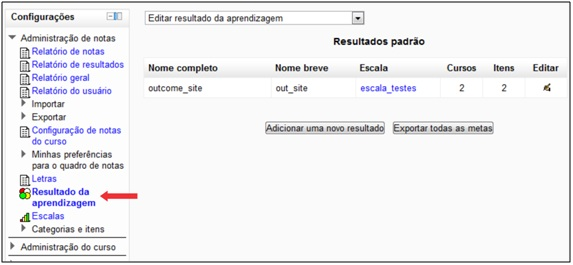
\includegraphics[width=0.6\textwidth]{imagem/cap6/fig21.jpg}}
  \caption{Adicionar Resultado de Aprendizagem}
  \label{fig:cap6_21}
 \end{center}
\end{figure}
\begin{figure}[htbp]
 \begin{center}
 \fbox{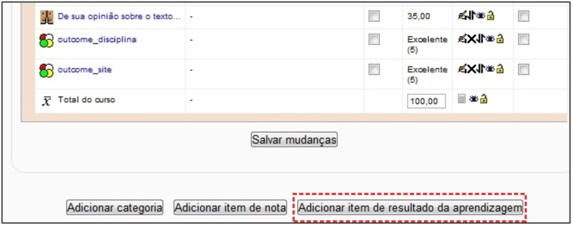
\includegraphics[width=0.6\textwidth]{imagem/cap6/fig22.jpg}}
  \caption{Botão adicionar item de resultado da aprendizagem}
  \label{fig:cap6_22}
 \end{center}
\end{figure}
\begin{figure}[htbp]
 \begin{center}
 \fbox{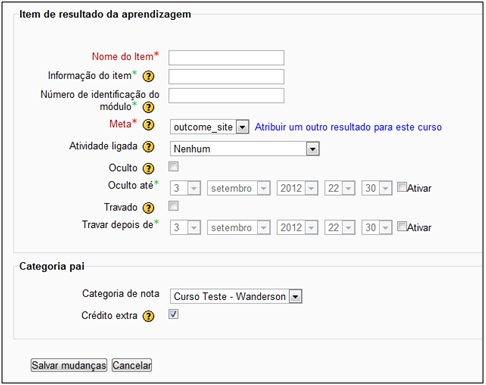
\includegraphics[width=0.6\textwidth]{imagem/cap6/fig23.jpg}}
  \caption{CConfiguração do Item de resultado da aprendizagem}
  \label{fig:cap6_23}
 \end{center}
\end{figure}

Novamente alguns campos apresentam a mesma funcionalidade dos itens anteriores (Adicionar categoria e item de nota), portanto, mantemos a mesma ideia citar as principais propriedades e opções do \textbf{Resultado de aprendizagem}.

\begin{itemize}
 \item \textbf{Nome do Item:} define o nome ou título do item de nota.
\item \textbf{Número de identificação do módulo:} definir uma identificação, que pode também ser uma abreviatura, é uma maneira de identificar a atividade para propósitos de cálculo na planilha de notas. Se a atividade não é utilizada em nenhum cálculo de notas, o campo pode ficar em branco. O número de identificação do módulo para um item de nota baseado em atividades é configurado na página de configurações das atividades.
\item \textbf{Meta:} especificar o resultado que o item de nota vai representar no relatório de notas. Conforme informado anteriormente, este resultado deve obrigatoriamente ser configurado na página de Resultado da aprendizagem, antes de ser vinculado a este item (Ver Figura 5.10). Somente resultados associados à disciplina ou ao Moodle da instituição podem ser usados.
\item \textbf{Atividade ligada:} é possível especificar ou não a qual das atividades da sua disciplina/curso este item de nota estará vinculado. Esta configuração pode ser utilizada para avaliar o desempenho do aluno em critérios não avaliados pelas notas nas atividades.
\item \textbf{Crédito extra (Categoria Pai):} quando a soma das notas é utilizada como estratégia de agregação, um item pode ser considerado crédito extra na categoria.
\end{itemize}

Ao retomarmos para página principal de Categoria e itens, sendo ela Visão Simples ou Completa, podemos fazer alterações de configurações diretamente na planilha de notas, configurações estas detalhadas anteriormente nos botões \textbf{Adicionar Categorias} e \textbf{Adicionar Itens de notas} e \textbf{Adicionar item de resultado da aprendizagem}, sendo que após realizar alterações, devemos clicar no botão \textbf{Salvar mudanças} para gravar as novas configurações da planilha.

\subsection{Exportar notas}

No Quadro de Notas da disciplina há um menu com barra de rolagem, na parte superior do relatório de notas. Ao abrir esse menu, clicando na seta lateral, entre outras opções podemos observar um grupo chamado \textbf{Exportar} (que também pode ser acessada através do bloco configurações). Veja a Figura \ref{fig:cap6_24}.

 \begin{figure}[htbp]
 \begin{center}
 \fbox{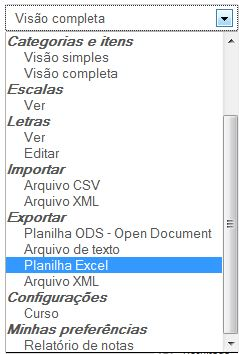
\includegraphics[width=0.3\textwidth]{imagem/cap6/fig24.jpg}}
  \caption{Exportar notas}
  \label{fig:cap6_24}
 \end{center}
\end{figure}
Temos quatro opções de exportação: Planilha ODS - Open Document; Arquivo de texto; Planilha Excel; Arquivo XML.

É importante salientar que, para exportar as notas dos alunos a tabela de notas não pode conter erros, ou seja, nenhuma coluna deve apresentar a palavra \textbf{erro}.

\subsection{Planilha Excel}
O Microsoft Office Excel (conhecido popularmente por Microsoft Excel) é um programa de planilha eletrônica escrito e produzido pela Microsoft para computadores que utilizam o sistema operacional Microsoft. O formato de arquivo exportado é .xls (1997-2003) e .xlsx (2007-atual). Atualmente é reconhecido por diversos aplicativos de planilha eletrônica, inclusive o BrOffice e OpenOffice.

Ao escolher a opção Exportar/Planilha Excel abrirá a tela configuração para exportação. Veja a figura abaixo.

 \begin{figure}[htbp]
 \begin{center}
 \fbox{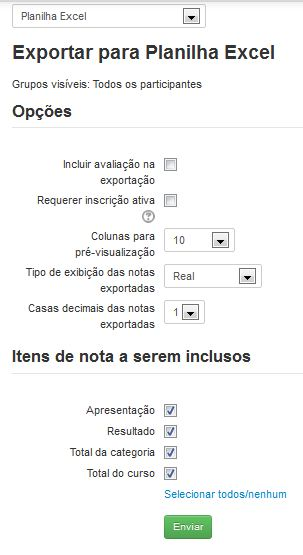
\includegraphics[width=0.3\textwidth]{imagem/cap6/fig25.jpg}}
  \caption{Exportar notas através da Planilha Excel}
  \label{fig:cap6_25}
 \end{center}
\end{figure}

Descrevemos abaixo o significado de cada item.
\textbf{Opções:}
\begin{itemize}
 \item Incluir avaliação na exportação: exporta as notas acompanhando o comentário do professor.
 \item Colunas para pré-visualização: estipula-se o número de colunas para pré-visualização da planilha antes de se realizar o download propriamente. Os valores são 10, 20, 100, 1000 e 100000.
 \item Tipo de exibição das notas exportadas: é possível escolher se a exportação das notas será pelo valor real, porcentagem ou letras.
 \item Casas decimais das notas exportadas: define o número de casas decimais das notas que serão exportadas.
\end{itemize}
\textbf{ Itens de nota a serem inclusos:}
\begin{itemize}
 \item Lista dos itens de nota: estarão listados aqui todos os itens de nota existentes no Quadro de Notas da disciplina com uma caixa de seleção ao lado. Embaixo dessa lista há dois links para Selecionar todos de uma vez ou Nenhum.
\end{itemize}
Após realizar as configurações, clicaremos em \textbf{Enviar}. Uma página de pré-visualização será exibida. Haverá um botão chamado \textbf{download}, ao clicar nele o arquivo no formato xls será salvo no computador. 
\section{Arquivo XML}
XML (\textit{Extensible Markup Language}) é uma linguagem de marcação padrão para inúmeros programas de computador. Por exemplo, ao converter um arquivo .DOC em PDF, usamos o XML do Word, onde estão todas as informações do documento que será convertido, em padrões que os outros aplicativos podem entender.

O XML usa uma sintaxe semelhante a Figura \ref{fig:xml}.

\begin{figure}[!htbp]
 \small
 \begin{center}
 \begin{tabbing}
   xxxx\=xxxx\=xxxx\=xxxx\=xxxx\=xxxx\=xxxx\=xxxx\=xxxx\=xxxx\= \kill
	<results batch="xml\_export\_1320693510">\\
    	\> <result>\\
    		\>\> <assignment>AP</assignment>\\
    		\>\> <student>aluno.teste01</student>\\
    		\>\> <score>$5.00$</score>\\
    	\> </result>\\
    </results>\\
  \end{tabbing}
 \end{center}  
 \caption{Exemplo Excel}
\label{fig:xml}
\end{figure}


Podemos notar que os números de identificação, tanto para as atividades como para os usuários, são fundamentais. Por isso a exportação do Quadro de Notas em XML precisa que todas as atividades e usuários tenham sua identificação configurada. O Moodle avisa isso antes da exportação.

Novamente, as configurações já mostradas no item Planilha ODS servirão aqui. Há somente um item extra (Tabela \ref{tab:XML}).

\begin{table}[htbp]
\begin{flushleft}
    \begin{tabular}{p{6cm}|p{9cm}} \hline
    \rowcolor[rgb]{0.8,0.8,0.8} \textbf{OPÇÕES} &  \\\hline
    \textbf{Exportacão nova ou apenas atualização de notas} & Escolher isso permite exportar somente as notas atualizadas, ou uma exportação nova do quadro inteiro. \\\hline

\end{tabular}
  \label{tab:XML}
  \end{flushleft}
\end{table}%

Ao clicar em Enviar uma página será aberta para conferência do conteúdo exportado e, clicando em \textit{download}, um arquivo XML pode ser aberto ou baixado para o computador do usuário. 

\section{Importar notas}

A importação de notas é utilizada para carregar um arquivo contendo avaliações de uma ou mais atividades e atualizar os valores da tabela de notas. É possível importar notas utilizando arquivos no formato CSV ou XML.

Um arquivo CSV é um formato de arquivo que armazena dados delimitados por um separador. Pode ser gerado, por exemplo, utilizando-se um editor de planilha eletrônica, como o Excel da suíte de aplicativos Microsoft Office. O XML já foi explanado anteriormente.

Para importar um arquivo de notas no formato CSV, basta clicar em Importar Arquivo CSV, conforme Figura \ref{fig:cap6_38}. A tela da Figura \ref{fig:cap6_39} será mostrada.

\begin{figure}[!htbp]
 \begin{center}
 \fbox{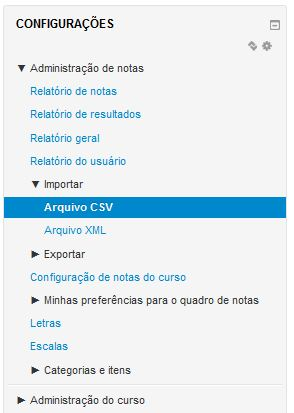
\includegraphics[width=0.3\textwidth]{imagem/cap6/fig38.jpg}}
  \caption{Importar notas}
  \label{fig:cap6_38}
 \end{center}
\end{figure}

\begin{figure}[!htbp]
 \begin{center}
 \fbox{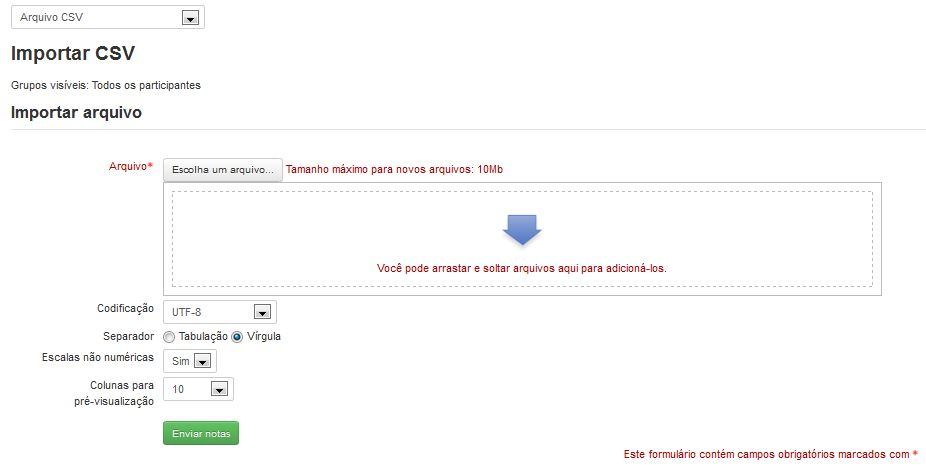
\includegraphics[width=0.6\textwidth]{imagem/cap6/fig39.jpg}}
  \caption{Importar notas através de arquivo CSV}
  \label{fig:cap6_39}
 \end{center}
\end{figure}

Para dar seguimento a este procedimento de importação é preciso ter um arquivo CSV configurado/editado adequadamente para que não haja inconsistências ou erros. Pode-se fazer isto utilizando a exportação de arquivo Excel, Open Document ou de texto, explicadas anteriormente, para ter um arquivo base. É preciso realizar as atualizações de nota desejadas e então salvar o arquivo como .csv ou .txt. Abra o arquivo utilizando um editor de texto simples para conferir se o separador que foi utilizado é tabulação ou vírgula, pois existem apenas estas duas opções para configuração de importação no moodle.

É preciso atentar também para a codificação para não haver inconsistências com o texto (nomes das atividades, comentários, etc). As demais opções podem ser deixadas como estão. A seguir clique em “Enviar notas”. Tomando um exemplo específico, na tela da Figura \ref{fig:cap6_40} vê-se o próximo passo de importação para o caso de o professor querer atualizar apenas as notas do Fórum de apresentação.

\begin{figure}[!htbp]
 \begin{center}
 \fbox{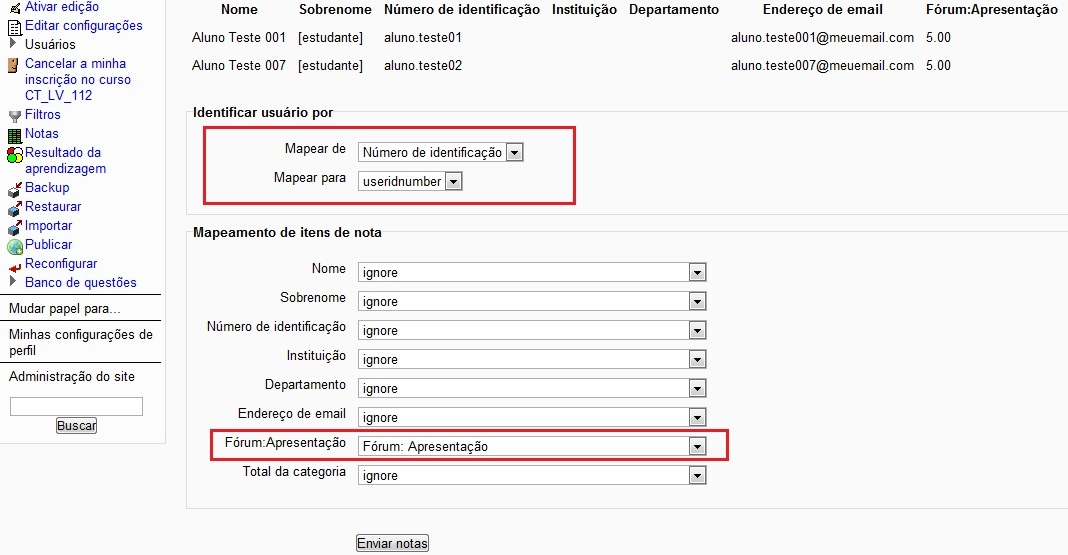
\includegraphics[width=0.6\textwidth]{imagem/cap6/fig40.jpg}}
  \caption{Importar notas apenas de Fóruns de apresentação}
  \label{fig:cap6_40}
 \end{center}
\end{figure}

É preciso especificar, na sessão “Identificar usuário por”, a forma como o moodle irá identificar corretamente cada usuário (correspondência biunívoca).  Pode-se utilizar qualquer campo, mas é importante ter certeza de que este seja único, por usuário. No exemplo, mapeou-se de “userIDnumber” para “Número de identificação”. 

A sessão “Mapeamento de itens de nota” também é utilizada pelo moodle para identificação biunívoca, mas para os itens de nota (observe que o total de uma categoria é tratado como item de nota). A fim de atualizar as notas do fórum de apresentação, faça a correspondência do item de nota com a coluna adequada da tabela, que no exemplo tem o mesmo nome.

Feito isto, clique em enviar notas para finalizar o processo de importação. 

É importante ressaltar que os nomes utilizados para mapeamento podem mudar de acordo com a tradução da instalação moodle para o português.

A importação de arquivo xml segue os mesmos passos da importação de arquivos CSV. Deve-se exportar um arquivo XML para servir de base, atualizar as notas com um editor adequado e fazer a importação. O passo a passo é descrito a seguir:

Clique em ‘Importar Arquivo XML’ no bloco configurações (Figura \ref{fig:cap6_41}).

\begin{figure}[!htbp]
 \begin{center}
 \fbox{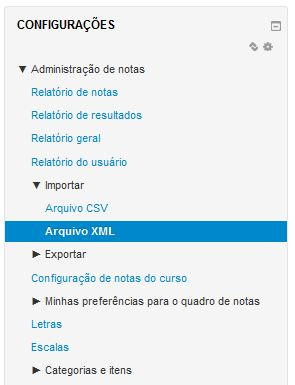
\includegraphics[width=0.3\textwidth]{imagem/cap6/fig41.jpg}}
  \caption{Importação de arquivo XML}
  \label{fig:cap6_41}
 \end{center}
\end{figure}

Após exportar um arquivo XML para utilizar de base, atualize-o com as notas desejadas. A atualização das notas pode ser feita utilizando um editor de texto simples ou um específico para este tipo de arquivo. Depois de editado o arquivo carregue-o no moodle através do botão “Escolha um arquivo” (Figura \ref{fig:cap6_42}).

\begin{figure}[!htbp]
 \begin{center}
 \fbox{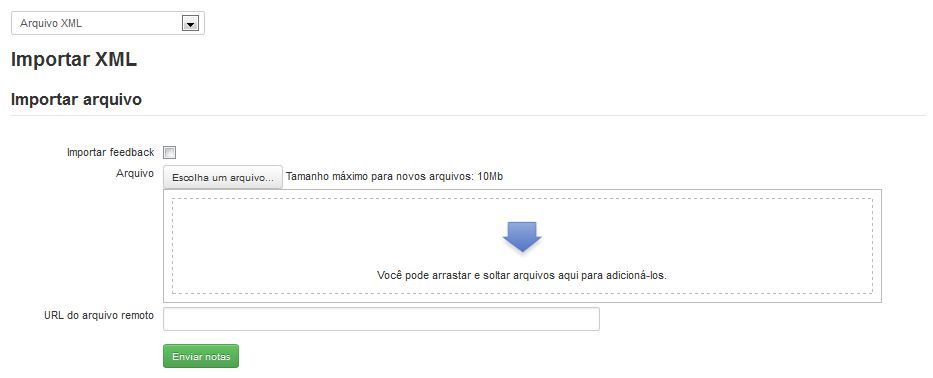
\includegraphics[width=0.6\textwidth]{imagem/cap6/fig42.jpg}}
  \caption{Escolhendo arquivo XML}
  \label{fig:cap6_42}
 \end{center}
\end{figure}


\begin{figure}[!htbp]
 \begin{center}
 \fbox{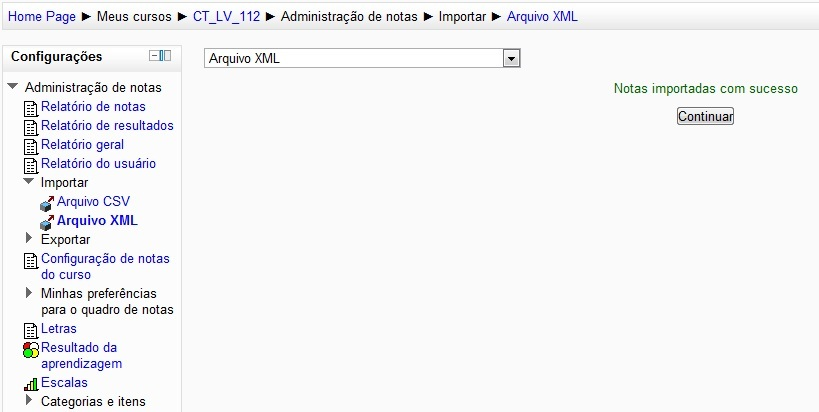
\includegraphics[width=0.6\textwidth]{imagem/cap6/fig43.jpg}}
  \caption{Confirmação de envio}
  \label{fig:cap6_43}
 \end{center}
\end{figure}


Feito isto, clique em “Enviar Notas”. Se tudo correu bem a seguinte tela será exibida (Figura \ref{fig:cap6_43}). 


No caso de arquivo XML, não há necessidade de mapeamento de usuários e itens de nota, pois o próprio arquivo contém informações suficientes para uma correspondência biunívoca. 